\documentclass{article}
\usepackage{graphicx}
\usepackage{python}
\begin{document}


\section{Introduction}


	\subsection{Client Identification}

 
		My Client is Paul Cox, a 54 year old mechanic. He has some experience with computers although not much. He uses computers for browsing, emails and using office programs 			such as word and excel for his business. He currently has a laptop running windows 7 64bit which he uses for this.
		Paul is a self-employed car mechanic who specialises in fixing SAABs but he also runs the rest of the business including billing, stock management and booking appointments with 			customers with occasional help from his wife, Karen Cox. 	
		The Garage is based in Cambridge but he often works at home, in Cottenham, when he is writing invoices or doing general tasks. 
		He would like to develop a system to store the data of their customers, to book appointments and help stock control.  He would like a database to store customer information so 			that he could access it from work or home without having to transport physical files.He would like to be able to enter the amount of time and the parts used into the system to use for invoices and then have the ability to print invoice.
		
		 \subsection{Define the current system}

		The client's current system is a physical filing system which stores files into a filing cabinet. This means that data can only be accessed from one place at a time, it is easily lost, 			put back into the wrong place or duplicate files can be made for the same customer.  
		There is also no backup so if it is damaged then the data is lost.  	
		The way they book appointments in is by using a diary and writing in when the customer is coming in. If this book is lost or damaged then they will have no way of knowing when customers have booked appointments. 
		
		Currently they record information about each individual job , this is a blank piece of paper that the the time spent, parts used and other costs that occured such as oil dumping the cost
		The current invoice system uses a book with a template that has to be manually filled in.
		

	\subsection{Describe the problems}
	
		There are many issues with the current system. First of all is the fact that information only has one copy and is stored with hundreds of other files, makes it hard to find quickly, 			easy to miss-place and easy to accidentally make duplicates of the same information. 
		Sometimes instead of updating their current file a new one will be added so a customer will have two files with different information on.

		Because the data is entered onto blank cards the format and type of data in each file can be inconsistent.

		The data is stored in a physical filing system and doesn't have any back ups. This means if the files are lost, damaged or stolen then the data is lost and will have to be manually 			recovered
		

		Another issue is that because appointments are currently stored in a diary so you can easily find appointments by date but not by the person they are with. This means that if a 			customer has forgotten the date of their appointment they will often

		The current invoice system is ok although human errors can occure since the information has to be manually entered and if a mistake is made an entirely new invoice has to be 			made since they can't be edited. Also since it is made by hand it can be hard to read for the customers.

This information is sourced from the current filing system
		mostly so if the information is not correct in the filing system then the invoice will be incorrect.


	\subsection{Section appendix}
		add later(proof) scan question sheet


\section{Investigation}

	\subsection{The current system}

	\subsubsection{Data sources and destinations}
		There are  two data sources in the current system, the client and the business.
		

\begin{tabular}{l|p{4cm}|p{4cm}|r}
\hline
Source & Data & Example & Destination\\ \hline
Client & First name, Last name, address, postcode, phone number, email & John Handcock, 1 The Road, Cambridge, cb4 1ab, 01223 0123456  & Filing system\\ \hline
Mechanic & Problem to be fixed & worn brake pads & appointment Diary\\ \hline
Mechanic & parts required & brake pads & supplier \\ \hline
Supplier & cost of parts & £8.50 & Task Sheet \\ \hline
Mechanic & Price and date of appointment & £35.00, 01/01/15 & Customer \\ 

\hline
\end{tabular}



	\subsubsection{Algorithms}
		There are currently several algorithms being used.
		

		


	\subsubsection{Data flow diagram}
	
	\begin{figure}[H]	
	
	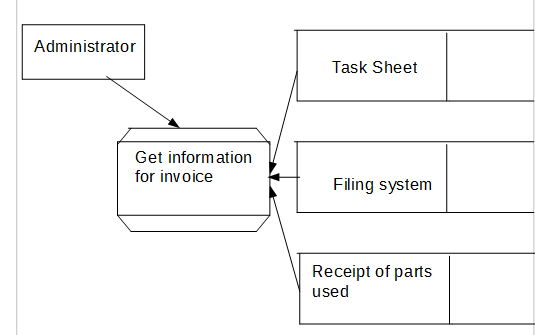
\includegraphics[width=\textwidth]{invoices.png}
    \caption{Invoices}
    
    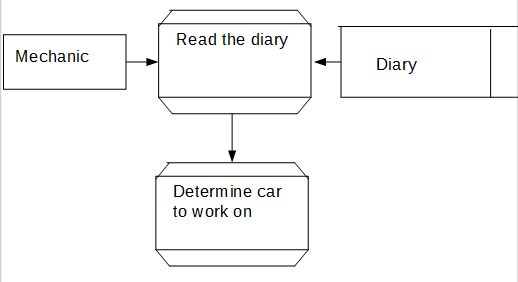
\includegraphics[width=\textwidth]{DeterminingWhatCarToWorkOn.PNG}
    \caption{Invoices}     
    
    \end{figure}
    
    \newpage
    
    \begin{figure}{H}
    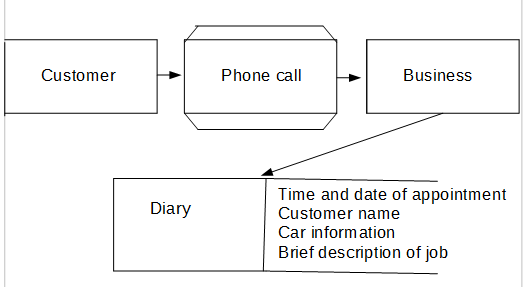
\includegraphics[width=\textwidth]{BookingJobsIn.PNG}
    \caption{hi}
    
    
    \end{figure}


	\subsubsection{Input Forms, Output Forms, Report Formats}
	
		\begin{figure}[H]
	
	
	
	  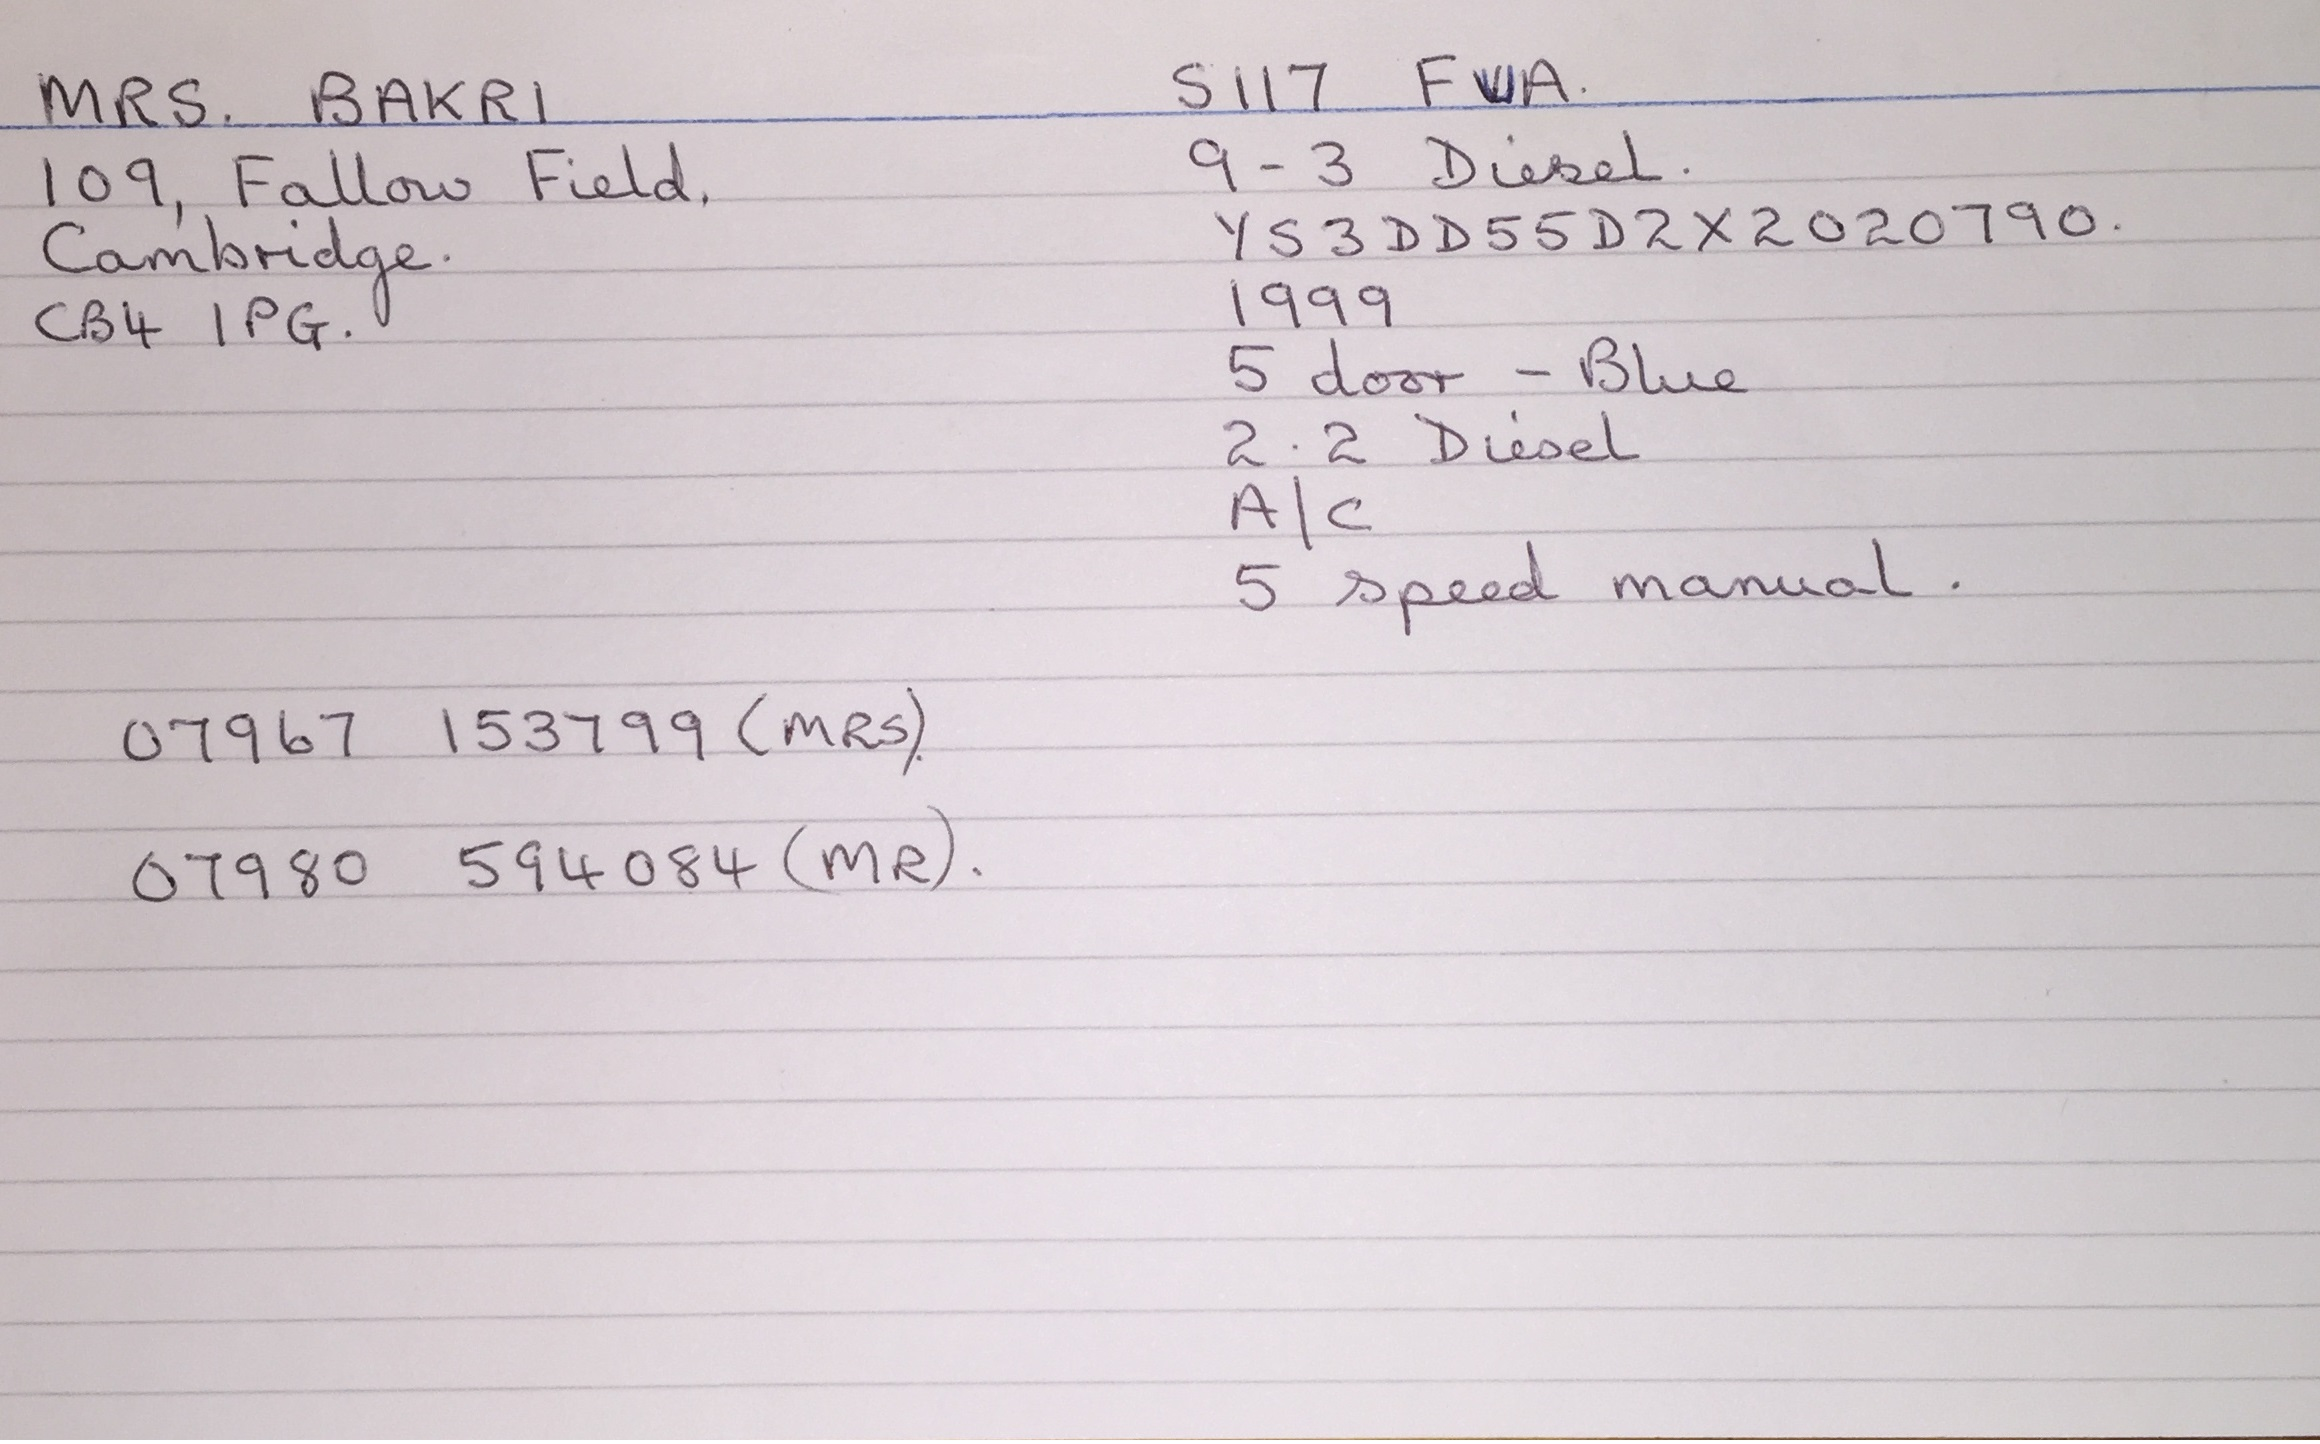
\includegraphics[width=\textwidth]{image_1.jpeg}
    \caption{This is an example of the part of the customers file that stores their address and car information.}
    
    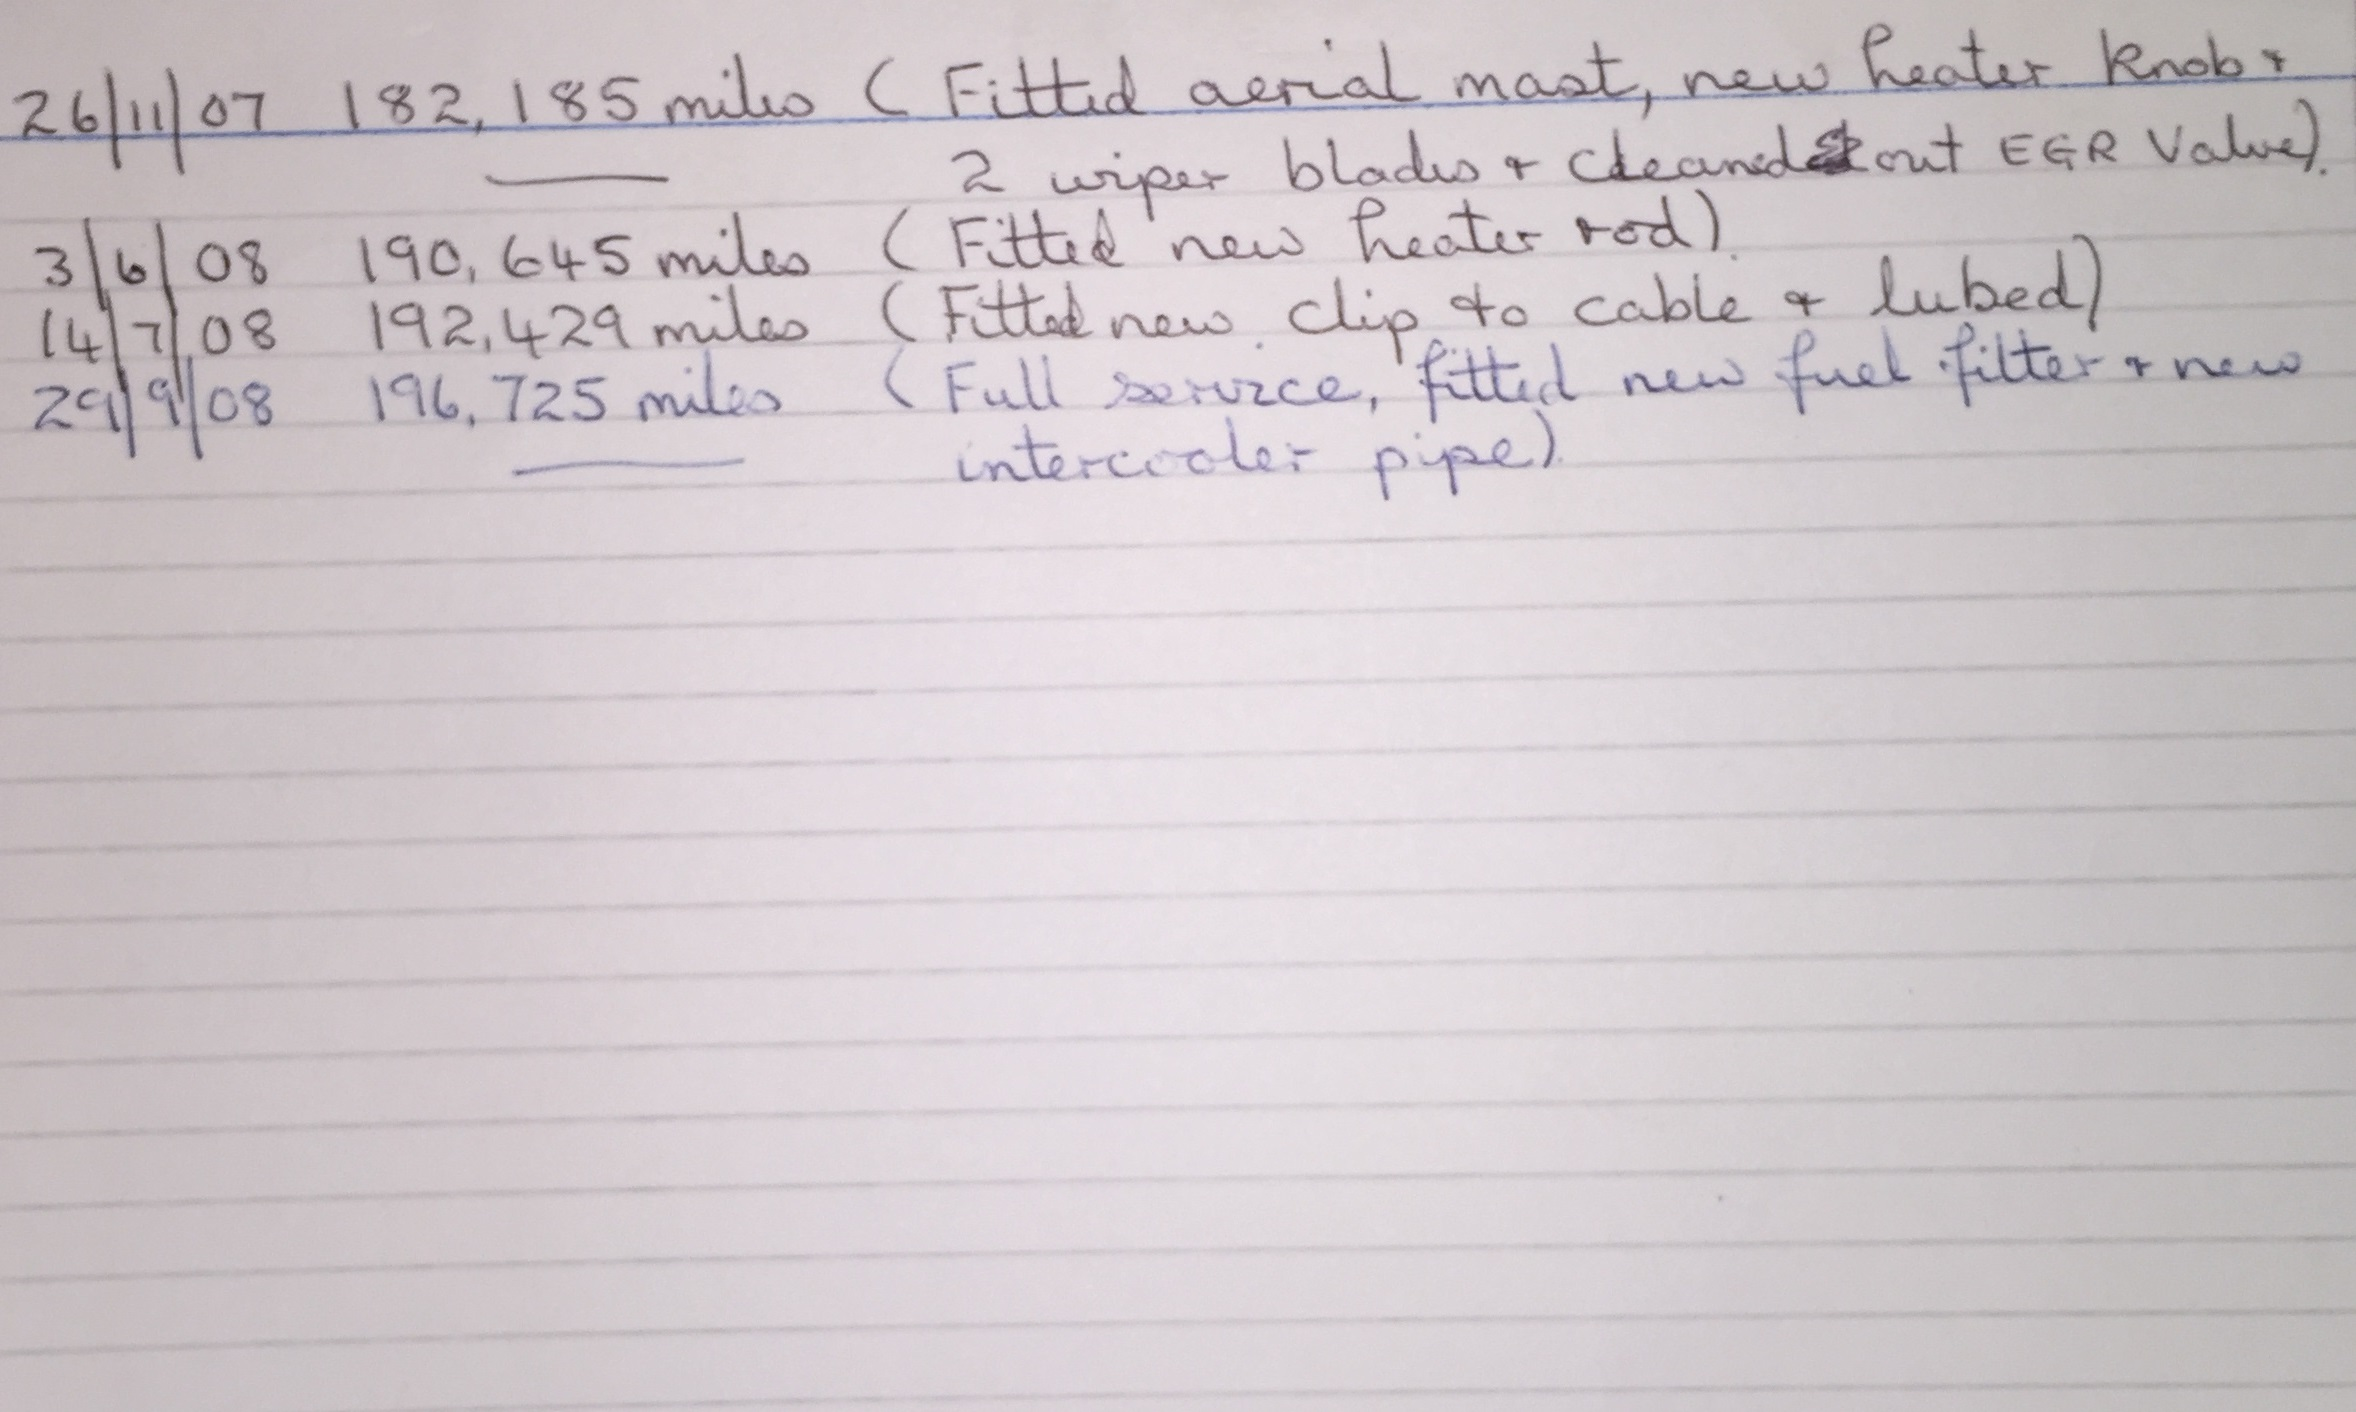
\includegraphics[width=\textwidth]{image_2.jpeg}
    \caption{This is an example of the part of the customers file that stores their service history}
    
    \end{figure}
    \newpage
	
	
	\begin{figure}[H]
    
    
    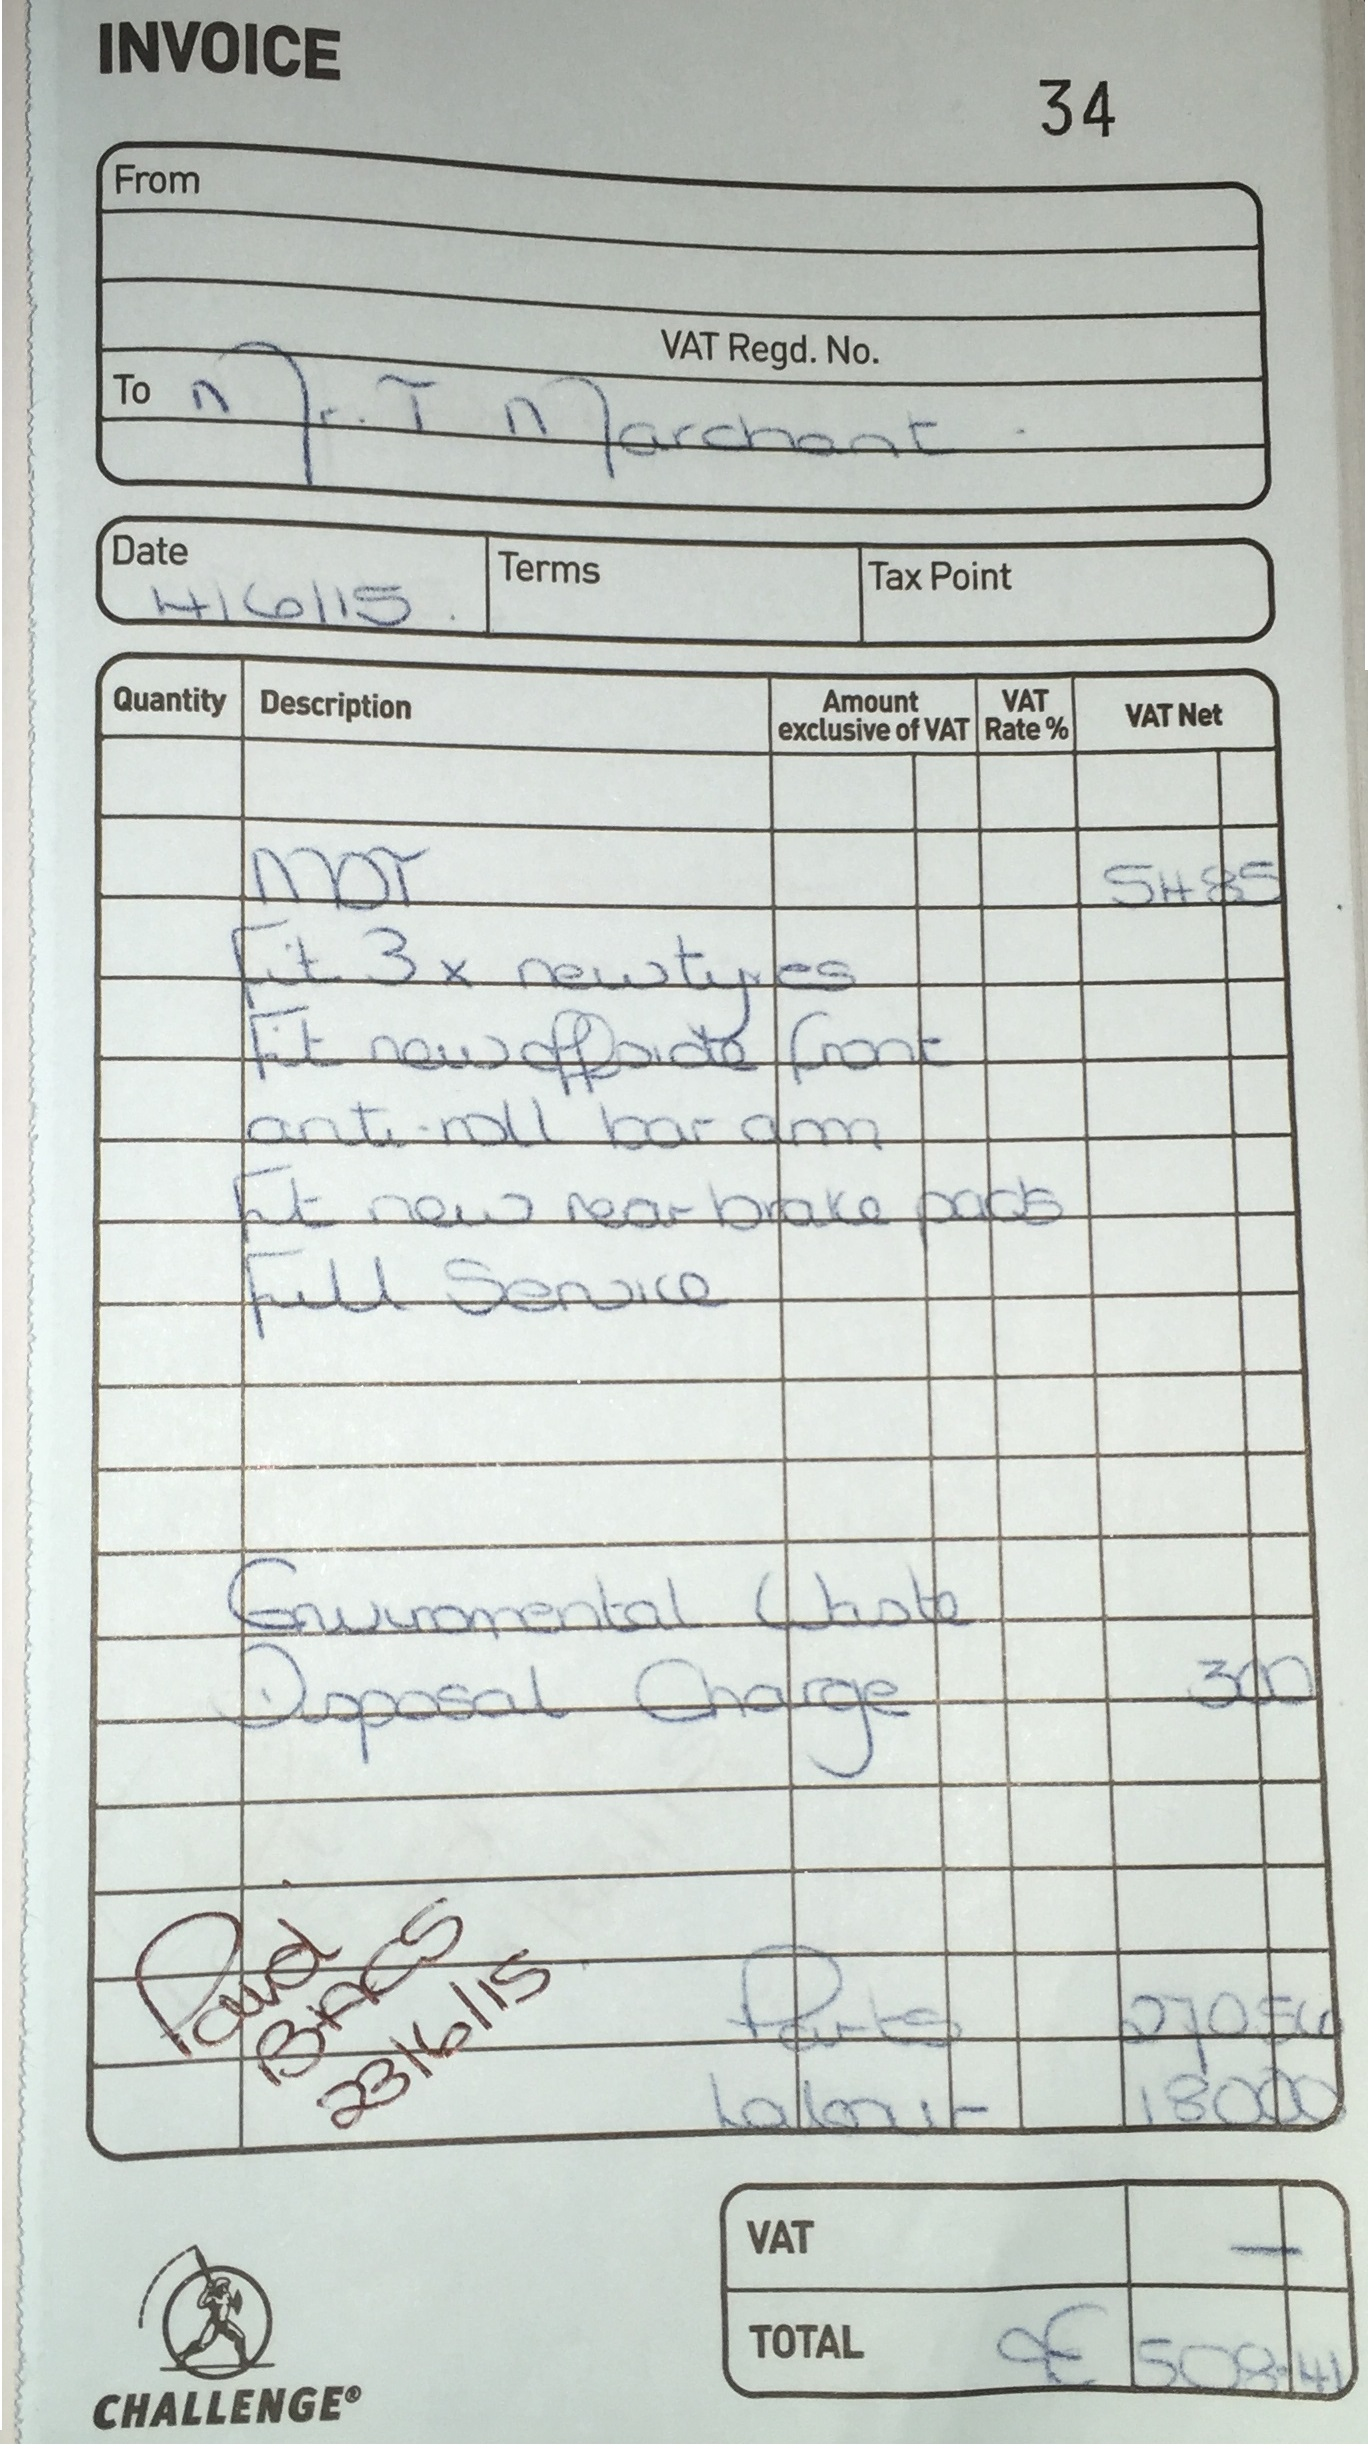
\includegraphics[width=\textwidth]{image_3.jpeg}
    \caption{This is an example of an invoice}
    
    \end{figure}
    \newpage
	
	
	\begin{figure}[H]   
    
    
    
    
    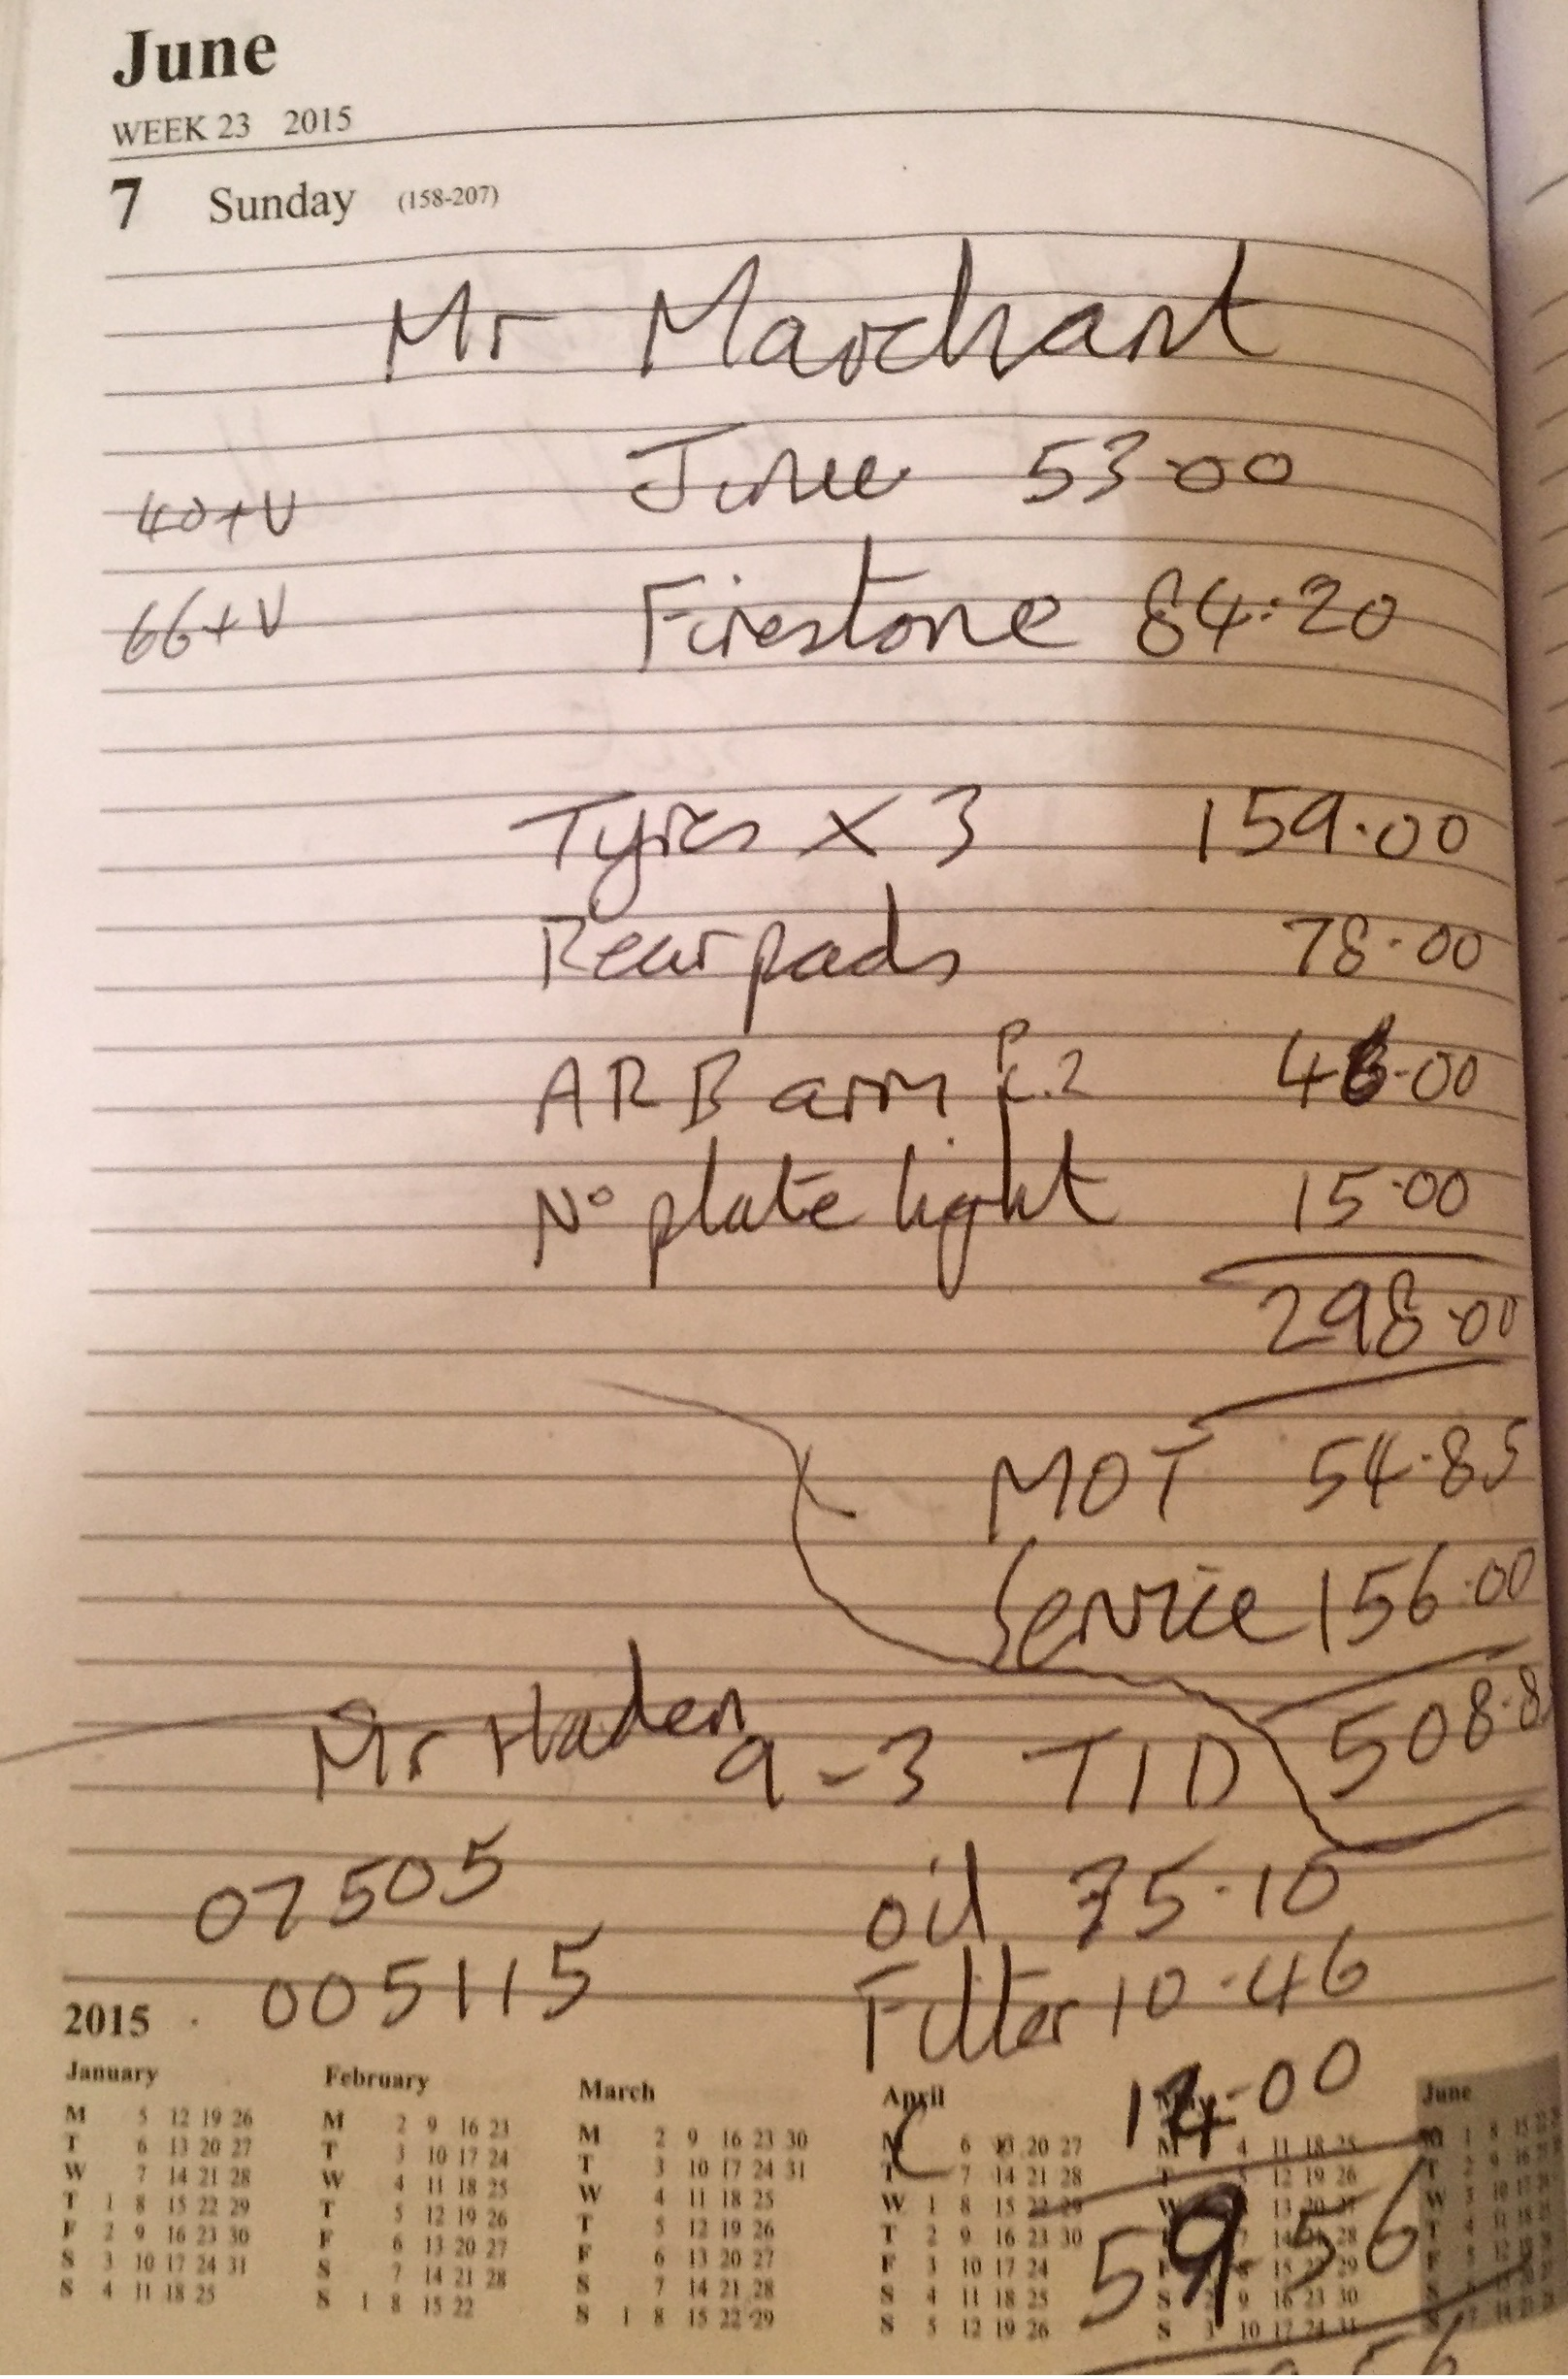
\includegraphics[width=\textwidth]{image_5.jpeg}
    \caption{This is an example of a diary entry that Paul uses to book appointments in}
    
    
	\end{figure}
	

	
		
	
	\subsection{The proposed system}
	

	\subsubsection{Data sources and destinations}

	\subsubsection{Data flow diagram}

	

	\subsubsection{Data dictionary}

	\subsubsection{Volumetrics}

		I have chosen an initial size of 300 files since he estimated he had around 500 customers so this will cover over half. he also said that he has anywhere from 1-4 customers a day(see interview) so this should cover him for around a year because he works around 250 days per year.

\section{Objectives}

	\subsection{General Objectives}
		Fast and easy to book appointments with customers
		
		to be able to access customer information quickly, clearly and easily.
		
		Be able to print out invoices.
		
		
		

	\subsection{Specific Objectives}

	\subsection{Core Objectives}

	\subsection{Other Objectives}

\section{ER Diagrams and Descriptions}

	\subsection{ER Diagram}
	
	\subsection{Entity Descriptions}

	\section{Object Analysis}

	\subsection{Object Listing}

	\subsection{Relationship diagrams}

	\subsection{Class definitions}

\section{Other Abstractions and Graphs}

\section{Constraints}

	\subsection{Hardware}

	\subsection{Software}

	\subsection{Time}

	\subsection{User Knowledge}

	\subsection{Access restrictions}

\section{Limitations}

	\subsection{Areas which will not be included in computerisation}

	\subsection{Areas considered for future computerisation}

\section{Solutions}

	\subsection{Alternative solutions}

	\subsection{Justification of chosen solution}


\end{document}